\documentclass{siamltex}
\usepackage{graphicx}
\usepackage{float}
\usepackage{subfig}
\usepackage{epsfig}
\usepackage{color}
\usepackage{epsf,amsmath,amssymb,amsfonts}
\newcommand{\ds}{\displaystyle}

%\usepackage[thinlines,thiklines]{easybmat}
%\textwidth = 14cm
%\oddsidemargin = 0pt
%\topmargin=0pt

%---------------------------------------------------------------------------
%
%          USER DEFINED MACROS
%
%\mathsurround = 2pt

\def \ds          {\displaystyle}
\def \rmd         {{\rm d}}
\def \be          {{\bf e}}
\def \bF          {{\bf F}}
\def \bI          {{\bf I}}
\def \bn          {{\bf n}}
\def \bff         {{\bf f}}
\def \bdf         {{\bf df}}
\def \bdT         {{\bf dT}}
\def \bT          {{\bf T}}
\def \cT          {{\cal T}}
\def \bU          {{\bf U}}
\def \bu          {{\bf u}}
\def \bv          {{\bf v}}
\def \bV          {{\bf V}}
\def \bX          {{\bf X}}
\def \by          {{\bf y}}
\def \bY          {{\bf Y}}
\def \bz          {{\bf z}}
\def \bZ          {{\bf Z}}
\def \bW          {{\bf W}}
\def \bZt         {{\bf \widetilde Z}}
\def \bzi         {{\bz}_i}
\def \bzs         {{\bz}^*}
\def \bzis        {{\bz}_i^*}
\def \bzin        {\{\bzi\}_{i=1}^k}
\def \cf          {{\cal F}}
\def \cg          {{\cal G}}
\def \ch          {{\cal H}}
\def \vi          {{V_i}}
\def \vin         {\{\vi\}_{i=1}^k}
\def \Babs        {{\Big|}}
\def \Bl          {{\Big(}}
\def \Br          {{\Big)}}
\def \Bleft       {{\Big[}}
\def \Bright      {{\Big]}}
\def \p           {\partial}
\def \R           {{\mathbb R}}
\def \N           {{\mathbb N}}
\def\y            {{\bf y}}
\def \tN          {{\widetilde{N}}}
\def \tD          {{\widetilde{D}}}

\def \proofnote #1{\footnote{{\bf Note: #1}}}
\def \norm      #1{\left\|\,#1\,\right\|}
\def \set       #1{\left\{\,#1\,\right\}}
\def \tr          {^T}
\def \IhH         {I_h^H}
\def \IhHb        {{\hat I}_h^H}
\def \IHh         {I_H^h}
\def \vbar        {\bar v}
\def \zhbar       {\bar z_h}
\def \zHbar       {\bar z_H}
\def \zhplus      {z_h^+}
\def \zHplus      {z_H^+}

\renewcommand{\theequation}{\thesection.\arabic{equation}}

\newtheorem{alg}{Algorithm}[section]
\newtheorem{thm}{Theorem}[section]
\newtheorem{lem}[thm]{Lemma}
\newtheorem{cor}[thm]{Corollary}
\newtheorem{pro}{Proposition}[section]
\newtheorem{defn}{Definition}[section]
\newtheorem{asp}{Assumption}[section]
\newtheorem{rmk}{Remark}[section]

%\def \Rblack#1{\,\hbox{R \kern-1.2em I
%    \kern.275em $^{#1}$}}
%\def \bG{{\bf G}}
%\def \bt{{\bf t}}
%\def \bzj{{\bz}_j}
%\def \bY{{\bf Y}}
%\def \byi{{\by}_i}
%\def \byj{{\by}_j}
%\def \byim{\{\byi\}_{i=1}^m}
%\def \bx{{\bf x}} 

%---------------------------------------------------------------------------

\title{\bf Truncated Newton-based multigrid algorithm for centroidal Voronoi diagram calculation}

\author{Zichao Di\thanks{Department of Mathematical Sciences, George Mason University,
  Fairfax, VA 22030. ({\tt zdi@gmu.edu})}
\and Maria Emelianenko\thanks{Department of Mathematical Sciences, George Mason University,
  Fairfax, VA 22030. ({\tt memelian@gmu.edu}).}
\and Stephen G.~Nash\thanks{Systems Engineering and Operations Research Department, George Mason University,
  Fairfax, VA 22030. ({\tt snash@gmu.edu}).
  }
}

\begin{document}

\maketitle


\begin{abstract}
In a variety of modern applications there arises a need to tessellate the domain into representative regions, called Voronoi cells. A particular type of such tessellations, called centroidal Voronoi tessellations or CVTs, are in big demand due to their optimality properties important for many applications. The availability of fast and reliable algorithms for their construction is crucial for their successful use in practical settings. This paper introduces a new multigrid algorithm for constructing CVTs that is based on the MG/Opt algorithm that was originally designed to solve large nonlinear optimization problems. Uniform convergence of the new method and its speedup comparing to existing techniques are demonstrated for linear and nonlinear densities for several 1d and 2d problems, and $O(k)$ complexity estimation is provided for a problem with $k$ generators.

\end{abstract}

\begin{keywords}
Optimal quantization, centroidal Voronoi tessellations,
Lloyd's algorithm, multilevel method, uniform convergence
\end{keywords}

\section{Introduction}\label{sec:1}

%Centroidal Voronoi tessellations are used in many applications such as image and data compression, pattern recognition,  image rendering  and so on \cite{Gray98}. They are used to tessellate a domain into representative regions, called Voronoi cells.  Centroidal Voronoi tessellations are a type of tessellation that is optimal in a particular sense.  For practical purposes, it is crucial to have fast and reliable algorithms to construct the tessellation.

A Voronoi diagram can be thought of as a map from the set of $N$-dimensional vectors in the domain $\Omega\subset\R^{N}$ into a finite set of vectors $\bzin$ called generators. It associates with each $\bzi$ a nearest neighbor region that is called a Voronoi region $\vin$. That is, for each $i$, $\vi$ consists of all points in the domain $\Omega$ that are closer to $\bz_i$ than to all the other generating points, and a Voronoi tessellation refers to the tessellation of a given domain into the Voronoi regions $\vin$ associated with a set of given generating points $\bzin\subset \Omega$ \cite{au90,Okabe}. With a suitably defined distortion measure, an optimal tessellation is given by a centroidal Voronoi tessellation, which is constructed as follows. For a given density function $\rho$ defined on $\Omega$, we may define the centroids, or mass centers, of  regions $\vin$ by
$$
\bzis =
\Bl
\int_{\vi} \y\rho(\y)\,d\y
\Br
\Bl
\int_{\vi} \rho(\y)\,d\y
\Br^{-1}.
 $$
 A {\em centroidal Voronoi tessellation} (CVT) is then a tessellation for which the generators of the Voronoi diagram coincide with the centroids of their respective Voronoi regions, in other words, $\bzi=\bzis$ for all $i$.

Given a set of points $\bzin$  and a tessellation $\vin$ of the domain, we may define the {\em energy functional} or the {\em distortion value} for the pair $(\bzin,\vin)$  by
$$ \label{ener}
{\cf}\Bigl(\bzin,\vin\Bigr)
=
\sum_{i=1}^k  \int_{\vi} \rho(\by)|\by - \bzi|^2 \,d\by.
$$
If the Voronoi tessellation $\vin$ is determined from $\bzin$ then we write
\begin{equation}
{\cg}\Bigl(\bzin\Bigr) \equiv {\cf}\Bigl(\bzin,\vin\Bigr).
\label{energy}
\end{equation}
The minimizer of $\cg$ necessarily forms a CVT which illustrates the optimization property of the CVT \cite{DFG}. This functional appears in many engineering applications and the relation of its minimizers with CVTs is studied, for instance, in \cite{Gersho, Gray98, Trushkin}. For instance, it provides optimal least-squares vector quantizer design in electrical engineering applications. The CVT concept also has applications  in diverse areas such as astronomy, biology, image and data analysis, resource optimization, sensor networks, geometric design, and numerical partial differential equations \cite{Cortes, DFG, DG02, DGJ02, DGJ03, DW1, DW3, Hiller03, JDG02, Mendes04, Brain04, Mesh04}. In \cite{DFG,DGJ10}, extensive reviews of the modern mathematical theory and diverse applications of CVTs are provided, %###
and this list is constantly growing.

The most widely used method for computing CVTs is the algorithm developed by Lloyd in the 1960s \cite{Lloyd}. Lloyd's algorithm represents a fixed-point type iterative algorithm consisting of the following simple steps: starting from an initial configuration (a Voronoi tessellation corresponding to an old set of generators), a new set of generators is defined by the mass centers of the Voronoi regions. The domain is re-tessellated and a new set of centroids is taken as generators. This process is continued until some stopping criterion is met. For other types of algorithms for computing CVTs we refer to \cite{au90,dwyer,for87,DGJ10}. It was shown that Lloyd's algorithm decreases the energy functional ${\cg}(\bzin)$ at every iteration, which gives strong indications of its practical convergence. Despite its simplicity, proving convergence of Lloyd's algorithm is not a trivial task. Some recent work \cite{DEJ, EJR} has substantiated  earlier claims about global convergence of Lloyd's algorithm, although single-point convergence for a general density function $\rho$ is still not rigorously  justified.

For modern applications of the CVT concept in large scale scientific and engineering problems such as data communication, vector quantization and mesh generation, it is crucial to have fast and memory-efficient algorithms for computing the CVTs. Variants of Lloyd's algorithm have been recently proposed and studied in many contexts for different applications \cite{DGJ02,Gray98,LBG,Gray86}. A particular extension using parallel and probabilistic sampling was given in \cite{JDG02} which allows efficient and mesh free implementation of Lloyd's algorithm. However, the issue of finding a better alternative remains critical for many applications, since Lloyd's algorithm and its variants are at best linearly convergent. Moreover, the standard Lloyd algorithm slows down as the number of generators gets large, which renders many practical calculations prohibitively expensive. Several alternatives have been proposed, including Newton-based methods \cite{DE06, Levy10} and GPU extensions \cite{Levy10_1, LNCS08}.

Multilevel algorithms present a desirable framework in the context of large-scale applications, since they do not suffer from the deterioration of convergence as the problem size grows---a typical pitfall of most iterative methods. The idea of multigrid and multilevel implementation of Lloyd's algorithm (referred to later as ``Multilevel-Lloyd method'') has been recently introduced in \cite{DE07}, where multigrid method was used as an ``outer" scheme, with Lloyd's algorithm playing the role of a relaxation at each level. The method was rigorously shown to be uniformly convergent for all smooth perturbations of a constant density in \cite{DE08} and was extended to the 2-dimensional setting in \cite{E10}, where it was successfully applied to a physical data binning application problems. Despite its uniform convergence, the method has a rather big computational cost for medium-sized problems and the construction of the interpolation operators is far from straightforward. An alternative approach was introduced by Yavneh et al. %### 
in \cite{yavneh03} that used a FAS (full approximation scheme) implementation of the Lloyd-Max scheme method based on minimizing the residual between generators and centroids. We refer to this algorithm as ``Multigrid Lloyd-Max method'' later in the text. Although successful in the 1-dimensional setting, this approach was not generalizable to higher dimensions \cite{yavneh06}.

Here we propose a new multilevel formulation for constructing CVTs in  the \sloppy 1-dimensional and %###
2-dimensional cases that is based on a different type of FAS scheme.  %###
Our approach is distinctive because the algorithm uses a fine-tuned version of the``off the shelf'' techniques instead of special purpose approaches. A distinctive feature of the new method is its close relationship with optimization problems.  This is accomplished by formulating Lloyd's algorithm as a minimization problem in terms of the energy functional ${\cg}(\bzin)$. We then apply a multilevel optimization framework called MG/Opt to this functional.

MG/Opt is a general framework for optimization when a hierarchy of approximate models is available.  MG/Opt was originally developed in the context of optimal control problems with PDE constraints, but is applicable to a broader class of problems.  By choosing appropriate interpolation operators, we design a new scheme which enjoys uniform convergence with respect to the problem size similar to the aforementioned algorithms. The advantage comparing to the Multilevel-Lloyd method comes in a form of significant reduction of computational costs, while lower convergence factors and generalizability to higher dimensions favorably distinguishes it from the Multigrid Lloyd-Max method.

Although MG/Opt is inspired by FAS, it is not equivalent to FAS.  In the simplest case, i.e., when MG/Opt is applied to an unconstrained problem, the update to the variables is the same as if FAS were applied to the first-order optimality conditions.  However MG/Opt includes a line search which guarantees convergence in the sense that $\ds \lim_{i\rightarrow \infty} \norm{\nabla \cg} = 0$. Even if a line search %###
is added to FAS, then FAS is only guaranteed to find a local minimizer of $\norm{\nabla \cg}$, which is not guaranteed to be zero.  Thus MG/Opt has stronger convergence properties than FAS.  In addition, MG/Opt (but not FAS) can be applied to optimization problems with constraints, such as bounds on the variables or more complicated constraints \cite{Nash10a}.  We expect this to be an important factor when applying MG/Opt to two- and higher-dimensional problems.  Additional reasons for preferring MG/Opt to FAS are discussed in \cite{LeNa05a}.

The rest of the paper is organized as follows. In section 2, we discuss the MG/Opt algorithm which forms the basis for the new CVT construction method. Its connection with the CVT formulation is the subject of Section 3, where we also introduce the new FAS implementation and define the corresponding operators. The results of numerical experiments and comparison with other methods are presented in Section 4, and final conclusions and discussion are found in Section 5.

\section{The Multilevel Optimization Algorithm}

We are applying a multilevel optimization algorithm called MG/Opt to the CVT problem. MG/Opt was originally developed to solve unconstrained optimization problems \cite{Nash00a}, with an emphasis on discretized optimization models.  It has been extended to constrained problems \cite{Nash10a} and the approach can be applied to problems not based on discretization.

MG/Opt is designed to accelerate a traditional optimization algorithm applied to a high-fidelity problem by exploiting a hierarchy of coarser models.  In its raw form it is an optimization framework, not an algorithm, since it depends on an underlying (traditional) optimization algorithm, here labeled ``OPT''. There is considerable flexibility in selecting the underlying optimization algorithm.  Of course, the performance of MG/Opt will depend on the choice of OPT.  MG/Opt is based on the ideas of the full approximation scheme (see, e.g., \cite{McCo92a}) but is not equivalent to the full approximation scheme.

Before giving a description of MG/Opt, it is necessary to say more about the underlying optimization algorithm OPT.  It is assumed that OPT is a convergent optimization algorithm in the sense that, if appropriate assumptions on the objective function $\cg$ are satisfied then
$$
\lim_{j\rightarrow \infty} \norm{\nabla \cg(\bz_j)} = 0
$$
where $\set{\bz_j}$ are the iterates computed by OPT.  (See, for example, \cite{GrNaSo08a}.)  We will write OPT as a function of the form
$$
\bz^+ \leftarrow \mbox{Opt}(\cg(\cdot),\bv,\bar \bz,k)
$$
which applies $k$ iterations of the convergent optimization algorithm to the problem
$$
\min_{\bz} \cg(z) - \bv\tr \bz
$$
with initial guess $\bar \bz$ to obtain $\bz^+$.  If the parameter $k$ is omitted, the optimization algorithm continues to run until its termination criteria are satisfied.  If OPT is applied by itself to the high-fidelity model, then $v = 0$.  In the context of the multilevel algorithm MG/Opt, non-zero choices of $v$ will be used.

To describe an iteration of MG/Opt we make reference to a high-fidelity model $\cg_h$ and a low-fidelity model $\cg_H$.  The letters $h$ and $H$ are used repeatedly to identify the high- and low-fidelity information.  Also required are a downdate operator $\IhH$ and an update operator $\IHh$ that map sets of generators $\bz$ from one level to another.  Unlike the algorithm in \cite{Nash10a}, the version of MG/Opt here uses a separate downdate operator $\IhHb$ to map values of $\nabla \cg$ from the fine level to the coarse level.

Here is a description of MG/Opt:
Given an initial estimate of the solution $\bz_h^0$ on the fine level, set $\bv_h = 0$.  Select non-negative integers $k_1$ and $k_2$ satisfying $k_1+k_2>0$.  Then for $j = 0, 1, \ldots$, set
$$
\bz_h^{j+1} \leftarrow
\mbox{MG/Opt}(\cg_h(\cdot),\bv_h,\bz_h^j)
$$
where the function MG/Opt is defined as follows:

\begin{itemize}
\item {\em Coarse-level solve:}  If on the coarsest level, then solve the optimization problem:
$$
\bz_h^{j+1} \leftarrow
\mbox{Opt}(\cg_h(\cdot),\bv_h,\bz_h^j).
$$
Otherwise,
\item {\em Pre-smoothing:}
$$
\bar \bz_h \leftarrow \mbox{Opt}(\cg_h(\cdot),\bv_h,\bz_h^j,k_1)
$$
\item {\em Recursion:}
\begin{itemize}
\item Compute
\begin{eqnarray*}
\zHbar &=& \IhH\zhbar \\
\vbar &=& \IhHb \bv_h + \nabla \cg_H(\zHbar) - \IhHb\nabla \cg_h(\zhbar)
\end{eqnarray*}
\item Apply MG/Opt recursively to the surrogate model:
$$
\zHplus \leftarrow
\mbox{MG/Opt}(\cg_H(\cdot),\vbar,\zHbar)
$$
\item Compute the search directions $e_H = \zHplus - \zHbar$ and $e_h = \IHh e_H$.
\item Use a line search to determine $\zhplus = \zhbar + \alpha e_h$ satisfying $\cg_h(\zhplus) \le \cg_h(\zhbar)$.
\end{itemize}
\item {\em Post-smoothing:}
$$
\bz_h^{j+1} \leftarrow \mbox{Opt}(\cg_h(\cdot),v_h,\bz_h^+,k_2)
$$
\end{itemize}

Because the integers $k_1$ and $k_2$ satisfy $k_1+k_2>0$, each iteration of MG/Opt includes at least one iteration of the convergent optimization algorithm OPT.  This fact, in combination with the line search to determine $\zhplus$, makes it possible to prove that MG/Opt is guaranteed to converge in the same sense as OPT  \cite{Nash10a}.

In this paper, we have chosen OPT to be the truncated-Newton algorithm TN \cite{Nash84sw}.  When applied to an optimization problem of the form
$$
\min_\bz f(\bz),
$$
at the $j$-th iteration a search direction $p$ is computed as an approximate solution to the Newton equations
$$
\nabla^2 f(\bz_j) p = -\nabla f(\bz_j)
$$
where $\bz_j$ is the current approximation to the solution of the optimization problem.  The search direction $p$ is computed using the linear conjugate-gradient algorithm.  The necessary Hessian-vector products are estimated using finite differencing.  The TN algorithm only requires that values of $f(\bz)$ and $\nabla f(\bz)$ are computed.  TN has low storage requirements, and has low computational costs per iteration, and hence is suitable for solving large optimization problems \cite{NaNo91a}.

\section{Applying MG/Opt to the CVT Formulation}

To make sure we are dealing with the same underlying problem on different levels, we scaled the objective function value by $k^{2}$ so that the optimal energy value would be same on every level for the uniform density. This  is also approximately true for other density functions.  The coarser grids were obtained by standard coarsening, i.e. doubling grid size at every level:  $N_H= \frac{1}{2}N_h$, where $N_h$ and $N_H$ are the numbers of grid points at the finer and coarser grids, respectively.

To define our algorithm for solving the CVT problem, we need to adapt the formulation above to the CVT context and specify the appropriate choices of the operators and algorithm parameters. It turns out the following choice of the transfer operators works best in the CVT MG/Opt context. Transfer of the solution from finer to coarser grid (error restriction) is done via simple {\em injection}, i.e. given a vector $\bv_h$ on the fine level, the downdate operator $\IhH$ samples $\bv_h$ at the even indices:
$$
[\IhH v_h]^{i}=v_h^{2i},\quad i=1,2,\ldots,k/2.
$$
The corresponding downdate operator $\IhHb$ for the gradient (gradient restriction) that maps values of $\nabla \cg$ from the fine level to the coarse level is given by
$$
[\IhHb v_h]^{i}=\frac{1}{2} v_h^{2i-1}+ v_h^{2i}+\frac{1}{2} v_h^{2i+1}, \quad i=1,2,\ldots,k/2.
$$
This form corresponds to the a standard choice of a full weighting (FW) restriction operator scaled by a factor of 2, which comes from scaling the objective function at each level. The update (interpolation) operator $\IHh$ is then given by a standard bilinear interpolation operator, which satisfies $\IHh =2(FW)\tr$ (see p.61 of \cite{trotten} for example), as is the case when solving an optimization problem based on a discretized PDE in one dimension. For our choice of the gradient restriction we obtain the relationship $\IHh=(\IhHb) \tr$, that we rely on in our implementation.

%According to \cite{trotten}, the factor 4 is necessary since the discrete operators $L_h$ and $L_{2h}$ have the different factors $h^{-2}$ and $(2h)^{-2}$. So the factor 4 has to be applied in the transfer of residual from the coarse to fine grid if apply full-weighting operator as restriction. So in order to work with same effect  but avoid giving a too large step of correction by applying update operator as 4 times of transpose of full weighting, we just balancely  use transpose of restriction as prolongation.

For a $V_{1,1}$ cycle implemetation, one pre-smoothing and one post-smoothing relaxations are used $k_1=k_2=1$, which corresponds to applying one iteration of OPT in each of these steps. We have tested several convergence criteria. As we demonstrate in Section \ref{num}, the best convergence was achieved when both OPT and MG/Opt were terminated due to saturation of the energy gradient $|\cg(\bz)-\cg(\bz^{*})| \le 10^{-8}$, where $\bz^{*}$ is the solution to the CVT problem.  The estimation of the exact solution $\bz^{*}$ was obtained by running OPT with a tight convergence tolerance.

It is also worth mentioning that we reordered the generators at each energy evaluation, since the order is not necessarily preserved by the optimization procedure described above. The symmetry of the CVT energy $\cg$ with respect to re-orderings of the points $\bzin$ assures that the objective function is not suffering from this modification.

\section{Numerical Experiments}
\label{num}

All numerical experiments have been performed on 2-core Intel Duo CPU E8400 3.00GHz platform with 3.25 GB of RAM and the running times might differ for other configurations.

We did not use any preprocessing to generate the starting configuration $\bz_h^0$ for our algorithm, which was simply obtained from a random sampling in the interval $[0,1]$. In Matlab, we reset the random generator seed each time and supplied the initial generators by means of the commands $\tt{rand('state',0), v0=sort(rand(k,1))}$ to eliminate the effect of initial configuration when benchmarking algorithm performance.

\subsection{1-dimensional examples}

All 1-dimensional examples have been computed on the $[0,1]$ domain. In the 1-dimensional case, the objective function (\ref{energy}) and its gradient can be integrated analytically in the case of $\rho=1$ and require numerical approximation for more complicated cases. For the types of nonlinear densities chosen in our numerical experiments we have tested several quadratures, including Simpson's and 15-point Gauss-Kronrod rules, with no significant change in algorithm performance.

In the numerical experiments below we compare the multilevel algorithm MG/Opt with the single level %###
counterpart (OPT) given by the Truncated Newton (TN) method. Since the TN algorithm is minimizing the %###
energy $\cg$ at every step, the approach is comparable %###
to the Lloyd algorithm (see \cite{DEJ}), which is the usual benchmark used for CVT algorithms.  We measure the computational cost of OPT by counting the number of fine-level gradient evaluations of $\cg$, which estimates the dominant cost of using OPT.  For MG/Opt we count the number of equivalent fine-level gradient evaluations.  That is, we determine (for each level) the relative cost of a gradient evaluation compared to an evaluation on the fine level.

Our first test uses the uniform density $\rho(y) = 1$ with $512$ variables.  This is an easy problem.  MG/Opt converges at a fast linear rate, about 12 times as fast as OPT  (see Figure \ref{fig:plot_evalgrad512}). Next we use the density $\rho(y)=6y^{2}e^{-2y^{3}}$.  The results are in Figure \ref{fig:plot_nonr512}.  In this case the performance of MG/Opt is almost the same, but OPT converges more slowly.  Again we are able to achieve fast linear convergence using the multilevel method. The convergence factor here is computed as follows:
\begin{equation}
\ds C=\Big(\frac{|\cg(\bz^{k+1})-\cg(\bz^{*})| }{|\cg(\bz^{1})-\cg(\bz^{*})| }\Big)^\frac{1}{k+1},
\label{C2}
\end{equation}
where $\cg(\bz^{*})$ is the approximation of the exact solution precomputed by running OPT until saturation.

\begin{figure}[h]
  \centering
  \subfloat[density $\rho(y) = 1$]
  {\label{fig:plot_evalgrad512}
  \includegraphics[width=2.5in]{plot_evalgrad512_1.jpg}}
  \subfloat[density $\rho(y) = 6y^{2}e^{-2y^{3}}$]
  {\label{fig:plot_nonr512}
  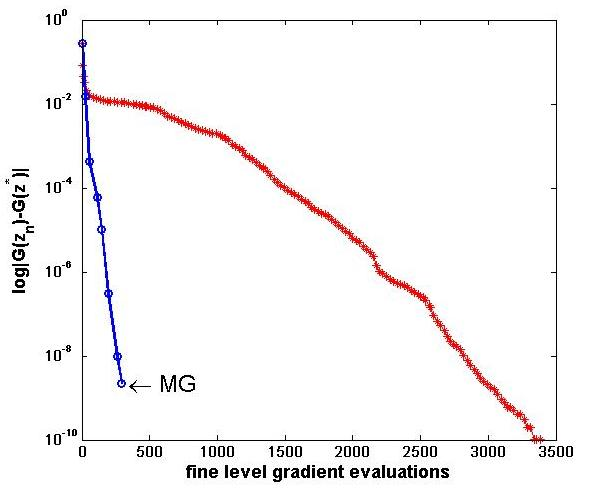
\includegraphics[width=2.3in]{nonlinear_eval512_1.jpg}}
  \caption{Comparison of MG/Opt versus OPT: (a) for density $\rho(y) = 1$, (b) density $\rho(y) = 6y^{2}e^{-2y^{3}}$.    Circle: MG/Opt, Star: OPT}
  \label{fig:unieval}
\end{figure}


In Figure \ref{fig:g_uni} we analyze the performance of MG/Opt and OPT as the size of the problem increases.  In these tests we used the uniform density $\rho(y) = 1$ and averaged the results over 6 independent runs with random initial guesses.  In the left plot we display the number of iterations needed for MG/Opt and OPT to compute the objective function value to a specified accuracy.  In the middle figure we display the time needed to do this.  Both MG/Opt and TN are expected to converge at a linear rate, and the rate constant (``convergence factor'') can be estimated from the results of each test.  The right plot displays the rate constants for both algorithms for different problem sizes.  As can be seen, for MG/Opt the rate constant is insensitive to the problem size, whereas for OPT the rate constant deteriorates as the problem size increases. Exact numerical values for both number of cycles, convergence factor and elapsed time are given in Table \ref{unitable}. Both MG/Opt and OPT algorithms have been stopped when the residual reaches a tolerance threshold of $10^{-8}$.

\begin{figure}[h]
\centering
  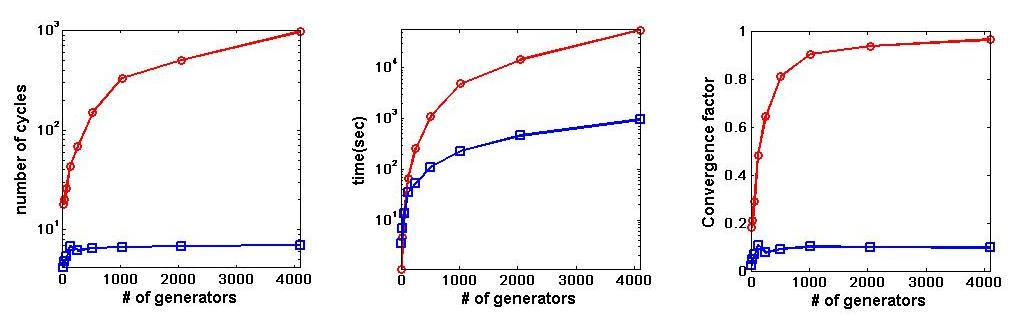
\includegraphics[width=1.0\textwidth]{ave_uni_mg_opt1.jpg}
%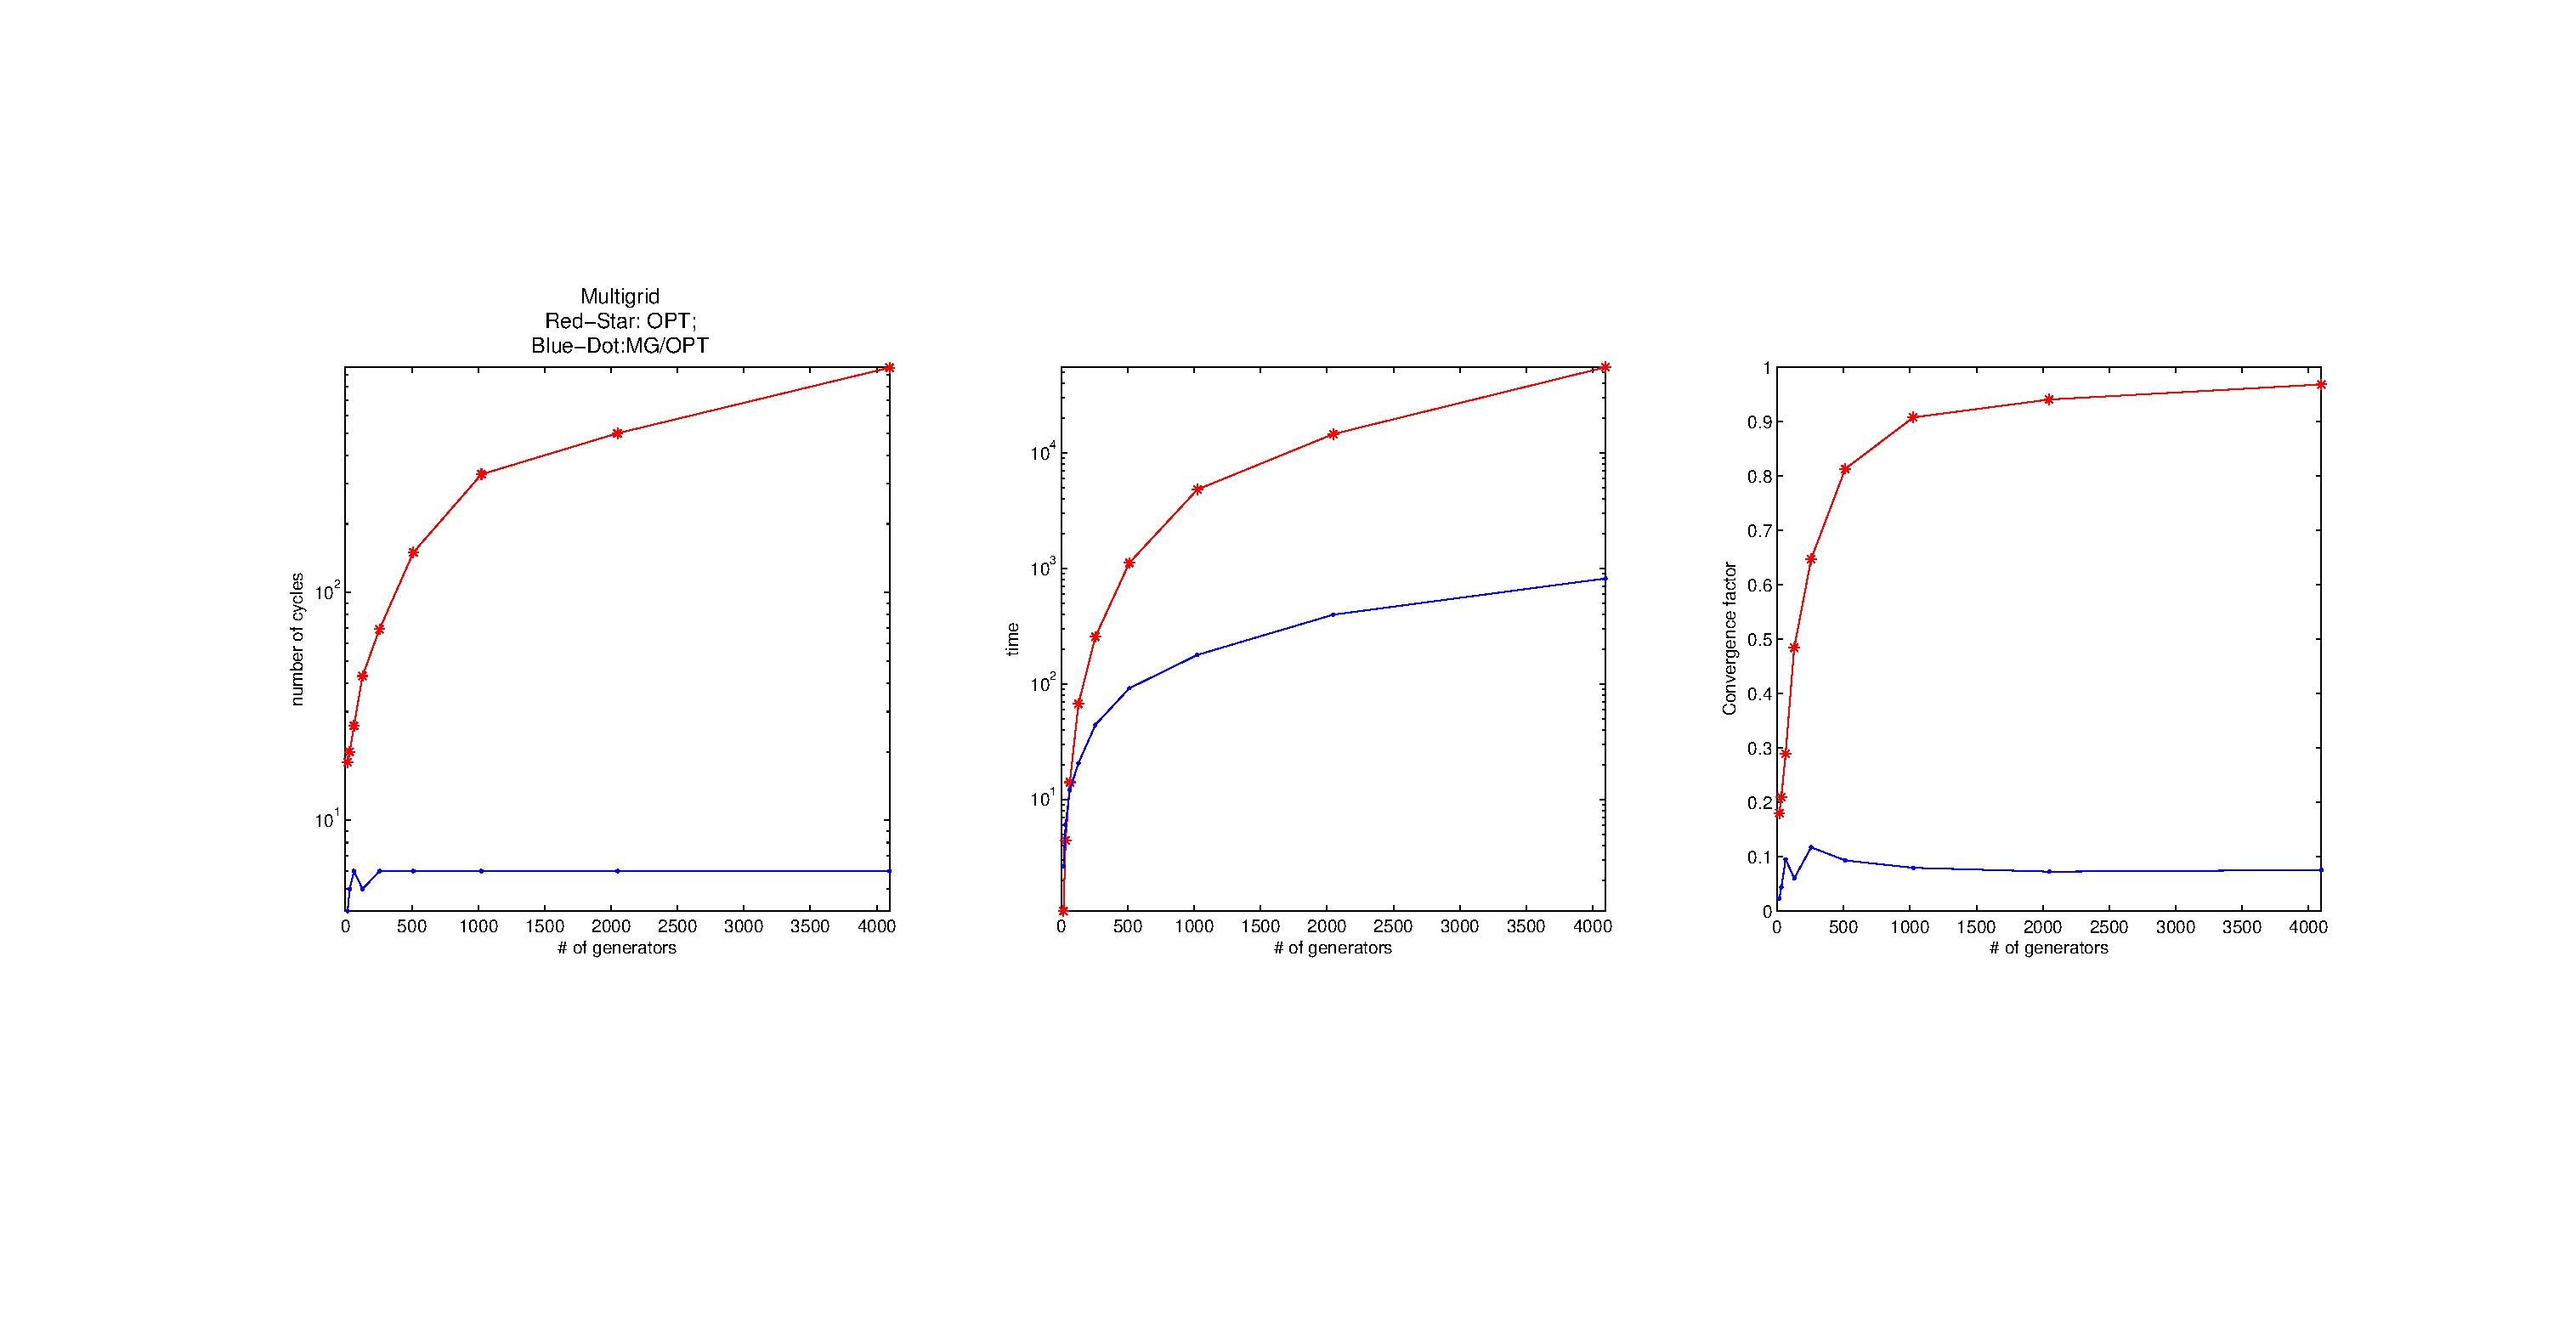
\psfig{file=graph_unioptmg.ps,width=1.0\textwidth}
  \caption{Solving problems of increasing size, MG/Opt versus OPT ($\rho(y) = 1$).  Blue-Square: MG/Opt, Red-Circle: OPT; Cycle numbers and Time elapsed are log scaled}
\label{fig:g_uni}
\end{figure}


\begin{table}
\begin{center}
%\resizebox{12cm}{3cm} {
\begin{tabular}{|l||l|l||l|l||l|l|} \hline
 &\multicolumn{2}{|c|}{convergence factor} &\multicolumn{2}{|c|}{number of cycles} &\multicolumn{2}{|c|}{time(sec)}\\ \hline
k& {\tt MG/Opt}&{\tt OPT}&{\tt MG/Opt}&{\tt OPT}&{\tt MG/Opt}&{\tt OPT}\\ \hline
16&0.0234&0.1803&4&18&2.63&1.08\\ \hline
32&0.0440&0.2094&5&20&6.02&4.44 \\ \hline
64&0.0952&0.2897&6&26&12.06&14.11 \\ \hline
128&0.0604&0.4839&5&43 &20.59&67.31\\ \hline
256&0.1174&0.6474&6&69&44.30&256.67 \\ \hline
512&0.0932&0.8129&6&150&91.73&1120.31 \\ \hline
1024&0.0796&0.9076&6&330&178.44&4831.66 \\ \hline
2048&0.0728&0.9403&6&500&398.56&14568.47 \\ \hline
4096&0.0757&0.9679&6&970&820.28&55370.94\\ \hline
 \end{tabular}
%}
\end{center}
\caption{Comparing performance of MG/Opt with 1-level optimization for $\rho=1$ }
\label{unitable}
\end{table}

Since the CVT algorithms in general show sensitivity 
to the choice of the initial configuration, we ran several tests with an intentionally ``bad'' %###
choice of the initial guess, with all generators clustered near the origin in the $[0,1]$ region. As Figure \ref{fig:bad} demonstrates, no significant difference in performance has been noted.

\begin{figure}[h]
\centering
  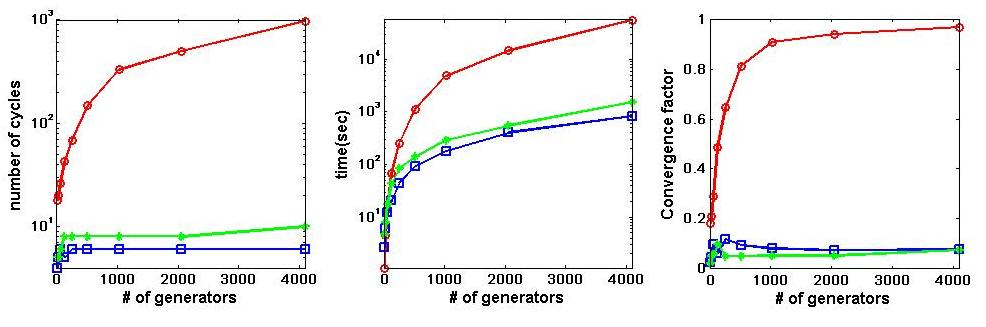
\includegraphics[width=1.0\textwidth]{uniopt_mg_bad_ini1}
  \caption{Performance of MG/Opt with different initial configurations. Red-Circle: OPT; Green-Star: MG/Opt with ``bad'' initial condition; Blue-Square: MG/Opt with random initial condition. Number of cycles and elapsed time axes are log-scaled.}
\label{fig:bad}
\end{figure}


Figure \ref{fig:g_difstop} shows the performance of MG/Opt when different stopping criteria are used.  Again we use the uniform density $\rho(y) = 1$.  From the plot, we can see that the common stopping criterion based on the improvement in the residual  $\nabla \cg$ (which is related to the difference between the positions of generators in the approximated and exact solution) is not the ideal choice here since it leads to a slight increase in the iteration count as the problem size increases.  For the other two criteria based on the energy function $\cg$, both the number of cycles and the convergence factors in MG/Opt are not sensitive to problem size. The other reason to prefer the criterion basen on energy values rather than positions is the abundance of local minima in the large-scale CVT problems, which makes it impossible to pinpoint the exact solution the method converges to. The energy value provides a reasonable measure for the closeness to a particular exact solution. However, as demonstrated by Figure \ref{fig:g_dfstop}, both criteria are acceptable and performance differences are minor.
It is also worth noting that based on the time complexity shown here the algorithm is linearly scalable --- a desirable feature %###
of the multigrid formulation that allows for an efficient parallelization for modern large-scale computing applications.

\begin{figure}[h]
\centering
  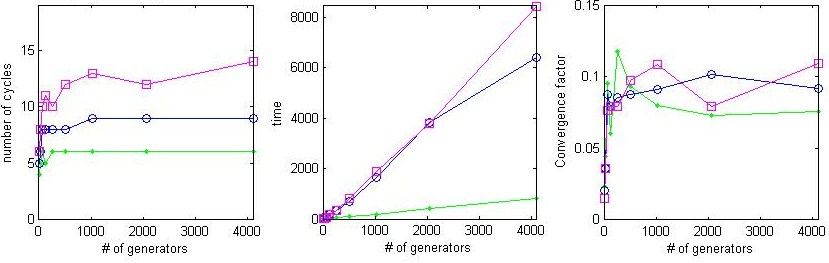
\includegraphics[width=1.0\textwidth]{uni_diffstop}
  \caption{Performance of MG/Opt with different stopping criteria ($\rho(y) = 1$).
    Blue-Dot: $|\cg(\bz)-\cg(\bz^{*})| \le 10^{-8}$; Red-Circle: $|\cg(\bz)-\cg(\bz^{*})| \le 10^{-11}$;
    Green-Square: $\norm{\nabla \cg}_\infty \le 10^{-6}$.}
\label{fig:g_difstop}
\end{figure}




Figure \ref{fig:g_difnon} demonstrates the performance of MG/Opt when applied to problems with different density functions.  In particular we consider $\rho_1(y)=1+0.1y$ and $\rho_2(y)=6y^{2}e^{-2y^{3}}$.  In the left plot, we can see that the iteration count for $\rho_1$ stays constant with the increase of the problem size, and increases only slightly for $\rho_2$.  For both densities the convergence factor exhibits insensitivity to the problem size, although the convergence factor is slightly larger for $\rho_2$, while remaining bounded from above by 0.2.


\begin{figure}[h]
\centering
  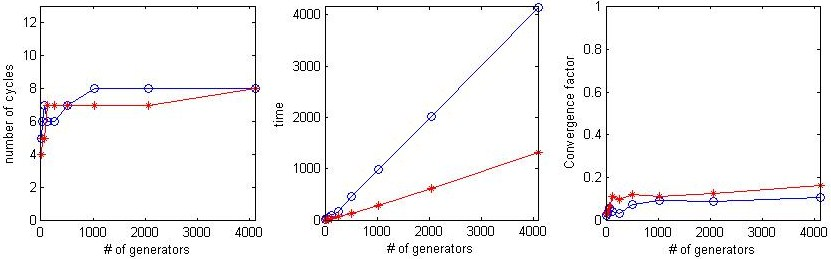
\includegraphics[width=1.0\textwidth]{diff_nonlgt}
  \caption{Performance of MG/Opt with different density functions.  Circle: $\rho(y) = 1+0.1y$.
    Star: $\rho(y) = 6y^{2} e^{-2y^{3}}$}
\label{fig:g_difnon}
\end{figure}

\begin{figure}[h]
\centering
  \subfloat[density $\rho(y) = 1$]
 { 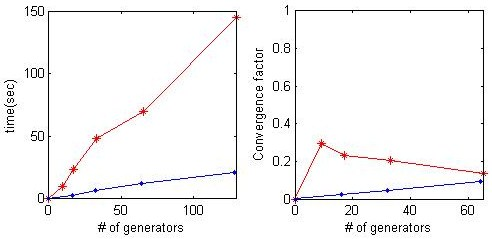
\includegraphics[width=3.5in]{uniform_mg_ml}}\\
  \subfloat[density $\rho(y) = 1+0.1y$]
 { 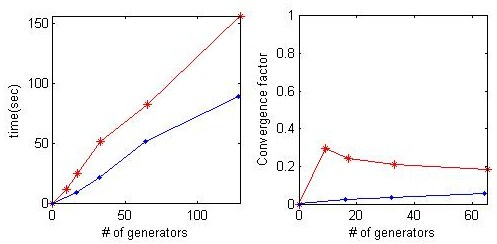
\includegraphics[width=3.5in]{linear_mg_ml}}
  \caption{Convergence factors for MG/Opt vs. Multilevel-Lloyd \cite{DE08} for (top)  uniform density $\rho(y) = 1$; (bottom)  linear density $\rho(y) = 1+0.1y$. Notations: Dot:MG/Opt; Star:Multilevel/Lloyd }
\label{fig:uni_ML}
\end{figure}

%\begin{figure}[h]
%\centering
%  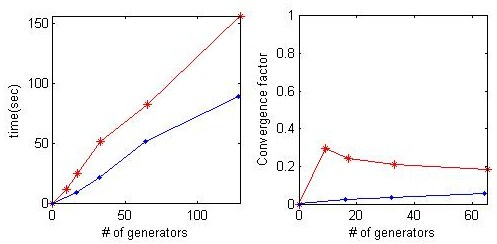
\includegraphics[width=4in]{linear_mg_ml}
%  \caption{Performance of MG/Opt vs. Multilevel-Lloyd \cite{DE08} for linear density $\rho(y) = 1+0.1y$. Dot:MG/Opt;
%   Star:Multilevel/Lloyd; Left: variable size vs. time; Right:variable size vs.convergence factor }
%\label{fig:lin_ML}
%\end{figure}

Figure \ref{fig:uni_ML}  compares the performance of MG/Opt to that of the multilevel optimization based method introduced in \cite{DE08}. Although the latter was also based on the idea of formulating an optimization problem based on the CVT energy (\ref{energy}), it has significant differences with the MG/Opt approach. Essentially, the previous scheme represented a successive correction algorithm with a suitably defined domain decomposition, with the Lloyd iteration used as a relaxation on each level --- hence %###
the name Multilevel-Lloyd we use to refer to it in this work. Comparison of performance of both methods for constant and linear densities shows that MG/Opt yields slightly lower convergence factors, while showing significant advantage in terms of the time complexity.




\begin{table}
\begin{center}
%\resizebox{11cm}{2.5cm} {
\begin{tabular}{| l |c | c | c | c | c |c |} \hline
 &\multicolumn{4}{|c|}{convergence factor} &\multicolumn{2}{|c|}{number of cycles }\\ \hline
k& ${\tt MG/Opt}^{2}$&${\tt MG/Opt}^{1}$&{\tt MLM}\cite{yavneh03}&{\tt OPT}&${\tt MG/Opt}^{2}$&{\tt OPT}\\ \hline
16&0.0350&0.0023&0.1725&0.8060&4&108\\ \hline
32&0.0314&0.0177&0.1782&0.9024&5&228 \\ \hline
64&0.0673&0.0551&0.1847&0.9381&5&354 \\ \hline
128&0.1120&0.0673&0.1962&0.9736&7&846 \\ \hline
256&0.0980& 0.0983 &    ---------    &0.9877&7&1818\\ \hline
512&0.1230&  0.1927         &---------   &0.9943&7&4276 \\ \hline
1024&0.1105&0.1504          & --------- &0.9971&7&8388\\ \hline
2048&0.1253&   0.2890          & ---------   &0.9983&7&14297 \\ \hline
 \end{tabular}
%}
\end{center}
\caption{Comparing performance of MG/Opt with 1-level optimization (OPT) and the Multilevel Lloyd-Max %###
(MLM) method of \cite{yavneh03} for a nonlinear density: $y=6x^{2}e^{-2x^{3}}$. %###
${\tt MG/Opt}^{1}$ denotes the MG/Opt algorithm with the convergence factor computed according to %###
(\ref{C1}), ${\tt MG/Opt}^{2}$ uses the geometric mean convergence factor (\ref{C2}); MLM\cite{yavneh03} is the result from \cite{yavneh03} with the same convergence factor formula as ${\tt MG/Opt}^{1}$ , 
`------' refers to data not provided in \cite{yavneh03}} %###
\label{mytable}
\end{table}

Table  \ref{mytable} compares the performance of MG/Opt with that of the OPT algorithm and the Multigrid Lloyd-Max (MLM) algorithm  introduced in \cite{yavneh03}, which is based on a FAS formulation of the Lloyd-Max iterative process. The same form of the nonlinear density $y=6x^{2}e^{-2x^{3}}$ as the one tested in \cite{yavneh03} has been chosen for fair comparison.  The column MG\cite{yavneh03} shows the convergence factors reported in \cite{yavneh03}, where the convergence factors were computed using
\begin{equation}
\ds C=\frac{|\cg(\bz^{k+1})-\cg(\bz^{*})| }{|\cg(\bz^{k})-\cg(\bz^{*})| }
\label{C1}
\end{equation}
The column ${\tt MG/Opt}^{1}$ lists the convergence factors for our algorithm MG/Opt computed the save way. The column ${\tt MG/Opt}^{2}$ lists the convergence factors for MG/Opt computed according to the formula (\ref{C2}), as we did in our earlier discussion. This latter formula is not as sensitive to the performance of the algorithm at the final iteration. It is also the formula used in our other numerical experiments when computing the convergence factor. Notice that the convergence factors for MG/Opt are significantly better than for MLM \cite{yavneh03}. The fact that convergence factors stay very small even for much larger problems  suggests that the new method has the potential to outperform earlier formulations, %###
even for highly nonlinear densities.

\subsection{2-dimensional examples.}
Below are some preliminary results that have been obtained in the 2-dimensional %###
case for the case of a triangular domain. %###

In Figure \ref{fig:2d_comp}, we give convergence results for MG/Opt and its competitors when the %###
initial guess is taken to be relatively close to the local minimizer. It is clear that MG/Opt maintains its superiority over OPT and Lloyd methods. Moreover, MG/Opt has a significantly lower convergence factors independent of the problem size, similar to the behavior observed in 1-dimensional case. Table %###
\ref{mytable2} provides numerical data for the performance of all three of these methods. Again, there is a clear advantage in using MG/Opt in this case. It has also been noted that the tendency of moving points outside of the domain typical for the regular 1-level OPT method is significantly reduced in the 2-dimensional MG/Opt implementation.

\begin{figure}[h]
\centering
  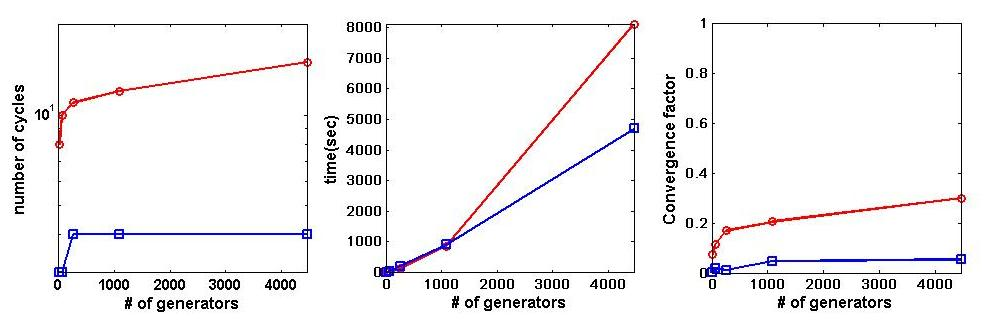
\includegraphics[width=1.0\textwidth]{comp_opt_mg_low1.jpg}
  \caption{Comparison of performance of MG/Opt, OPT and Lloyd for the case of a triangular 2-d %###
  region with $\rho=1$. Red-Circle: OPT, Blue-Square: MG/Opt.} %###
\label{fig:2d_comp}
\end{figure}

\begin{table}
\begin{center}
%\resizebox{11cm}{2.5cm} {
\begin{tabular}{| l |c | c | c | c  |c|c|} \hline
 &\multicolumn{3}{|c|}{convergence factor} &\multicolumn{3}{|c|}{number of cycles }\\ \hline
k &${\tt MG/Opt}$&{\tt OPT}&Lloyd & {\tt MG/Opt} &{\tt OPT}&Lloyd \\ \hline
 \end{tabular}
%}
\end{center}
\caption{Comparing performance of 2-dimensional MG/Opt with 1-level optimization (OPT) and Lloyd method for constant density in triangular domain. }
\label{mytable2}
\end{table}

Overall, while the above estimates are only a first step in a comprehensive analysis of the %###
2-dimensional version of the algorithm, and more work needs to be done to make the method work efficiently for general 2-d domains and density functions,  they give a reason to believe MG/Opt will be %###
competitive to other methods. Analysis of the performance of the 2-d method for different choices %###
of transfer operators, and the creation of a robust and versatile general-purpose solver are the %###
focus of current investigations.



\section{Complexity of MG/OPT for 1-d CVT problem}
In this section, we analyze the computational complexity of a $V_{1,1}$ cycle of the MG/Opt algorithm for CVT, i.e.  $k_1=k_2=1$. At each level, MG/Opt consists of Pre-smoothing and Post-smoothing which amount to two iterations of the Truncated Newton (TN) method, plus the cost of transferring the solution from one grid to another (downdate and update) and line search. Leaving the TN part aside, let us first compute the work required for all other parts of the algorithm, similar to the analysis performed in \cite{NaNo91a}. Notice that: (a) downdating the variables is carried out by means of simple injection, so no additional computational cost is involved; (b) the update operator is applied to half of the points in the grid %###
during the refinement process; (c) the process of downdating and finding local search directions is only applied to half of the points in the coarsening process; (d) these steps are performed in the beginning and at the end of each cycle. The setup is performed once per outer iteration. With these observations in mind, we obtain the estimate of computational cost for all these operations to be less than $9k$ for the problem of size $k$,  as shown in Table \ref{mgcom}.

\begin{table*}
\begin{center}
%\resizebox{10cm}{2cm} {
\begin{tabular}{|l||c|c||} \hline
Operations &per coordinate& on the fine level\\ \hline
Downdate(variable)&0&0\\ \hline
Downdate(residual)&3&$3k/2$\\ \hline
Search Direction&1&$k/2$\\ \hline
Update&3&$3k/2$\\ \hline
Line search&1&$k$\\ \hline
 \end{tabular}
%}
\end{center}
\caption{The complexity of various parts of MG/Opt measured in floating point operations.}
\label{mgcom}
\end{table*}

To estimate the complexity of the TN part, notice that if we only do one iteration of TN in pre-smoothing and post-smoothing, respectively, the following computations are to be performed:
\begin{itemize}
\item 1 infinity-norm calculation,  1 vector addition and 2 function-gradient evaluations
\item Conjugate-gradient (CG) iteration with cost per iteration given by:  \\1 function-gradient evaluation, \\4 inner product and \\5 ``vector + constant$\cdot$vector" operations.
\end{itemize}
 On average, we do 5 CG iterations per TN iteration.  Based on the above estimate, one TN iteration requires 1 infinity norm, 20 inner product, 25 ``vector + constant$\cdot$vector", 1 vector add calculations and 7 function/gradient evaluations. If the cost of infinity norm calculation is estimated to be no more that $k$ flops (floating-point operations, which include additions, subtractions, products and divisions), with $k$ being the number of grid points at the finest level, and the cost of each the inner product and ``vector + constant$\cdot$vector" calculations  is taken to be $2k$ flops, the overall cost of one TN iteration amounts to $ k (1 + 20 + 25 +1) = 47k$ flops, plus 7 function-gradient evaluations. Since in each $V_{1,1}$ cycle we do 2 TN iterations at each level and the contribution from coarser grids is estimated from above as $\sum^{\log k}_{i=0}{{2}^{-i}<2}$, we multiply this estimate by a factor of 4, and add the additional costs as specified above. We conclude that the typical cost of a MG/Opt V-cycle is $(4\cdot 47+9)k=197k$, plus $28k$ function-gradient evaluations.  This proves the fact that the above algorithm has $O(k)$ complexity. This bound can be lowered by performing less safeguarding as part of the TN algorithm at each step, however, we feel these steps are needed in order to obtain the most robust implementation.

\section{Comments and Conclusions}

In conclusion, we have introduced a novel way of computing CVTs by means of an $O(k)$ complexity algorithm based on the MG/Opt strategy originally used only for large-scale nonlinear optimization problems. %###
The main advantage of the new method is its superior convergence speed when compared to other existing approaches. Even though the computational complexity of each cycle is not the lowest, the fact that the convergence factors are on average much lower than those of its counterparts makes this formulation attractive when it comes to solving large CVT problems. The simplicity of its design and the results of preliminary tests suggest that the method is generalizable to higher dimensions, which is the subject of current investigations. Rigorous convergence theory development for this type of a method is nontrivial but possible, and will be addressed in a future publication. Future work also includes application of this technique to various scientific and engineering applications, including image analysis and grid generation.


\section{Acknowledgements}
The work of Zichao Di and Stephen G.~Nash was supported by the U.S.~Department of Energy under %###
Award DE-SC-0001691. Maria Emelianenko acknowledges the support from the ORAU Ralph E. Powe Junior %###
Faculty Enhancement Award.

%\bibliographystyle{unsrt}
\bibliographystyle{siam}
\bibliography{CVT_bib}

\end{document}
